\chapter{Ores and Energy in the Lithosphere}\label{ch:ores}
\chapterauthor{Marc Los Huertos and Alison Hong\footnote{Statement of Contributions: Alison Hong started this section with a provocative description of the issues with gold mining in the Phillipines. Later Los Huertos decided to put these mining activities in a geologic context and that could then be followed by a chapter on the formation and extraction of fossil fuels and the development of a population dependent on high density of energy.}}

\section{Energy: Industry, Food, and Population}

\subsection{Malthus and New Limits}

In the XXXX, Malthus argued that human population growth was exponential while resource growth was linear --- and a point had been reached where human populations would outstrip the capacity to get their basic needs met and misery would (or already had) fallen on the poor who would live destitute. He had some rather unsavory solutions to this conclusion --- stop feeding the poor with charity because they will just have more babies that would produce even more misery. 

In some ways, Malthus' observations remain and undercurrent in environmental views --- that humans will outstrip the resources of the Earth and even undermine the Earth's capacity to support non-human populations or even more poignant to many our own population.

However, in the late 1800s the predictions that humans would face a shortage of fire wood stimulated the US to take an active role in forest management to maintain a sustainable supply. However, with the use of coal and other fossil fuels humans were released from a carrying capacity on the Earth. In a strange way, then as discussed in the previous chapter, it is not the short supply of fossil fuels that might limit the development of human populations, but the waste product of this resource in the form of CO2 that will undermine our success as a species. 

\begin{figure}[h]
	\centering
		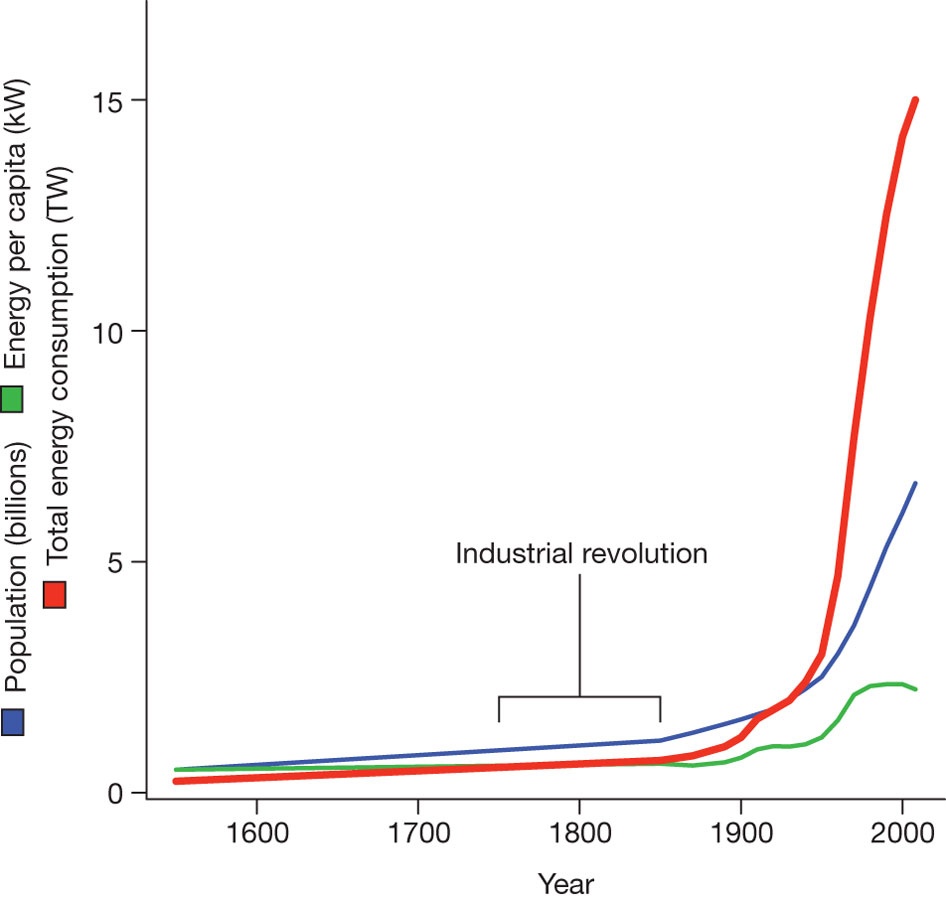
\includegraphics[width=1.00\textwidth]{graphics/energy_population.jpg}
	\caption{energy and population, demonstrating the changes -- although we need to be careful to not make assumptions to about causation --- correlation does not necessairly mean causation!}
	\label{fig:energy_population}
\end{figure}

In terms of the impact on the world, we have...the ``density of power'' demonstrates the value of fossil fuels (Figure~/ref{fig:Power-Densities}).

\begin{figure}[htbp]
	\centering
		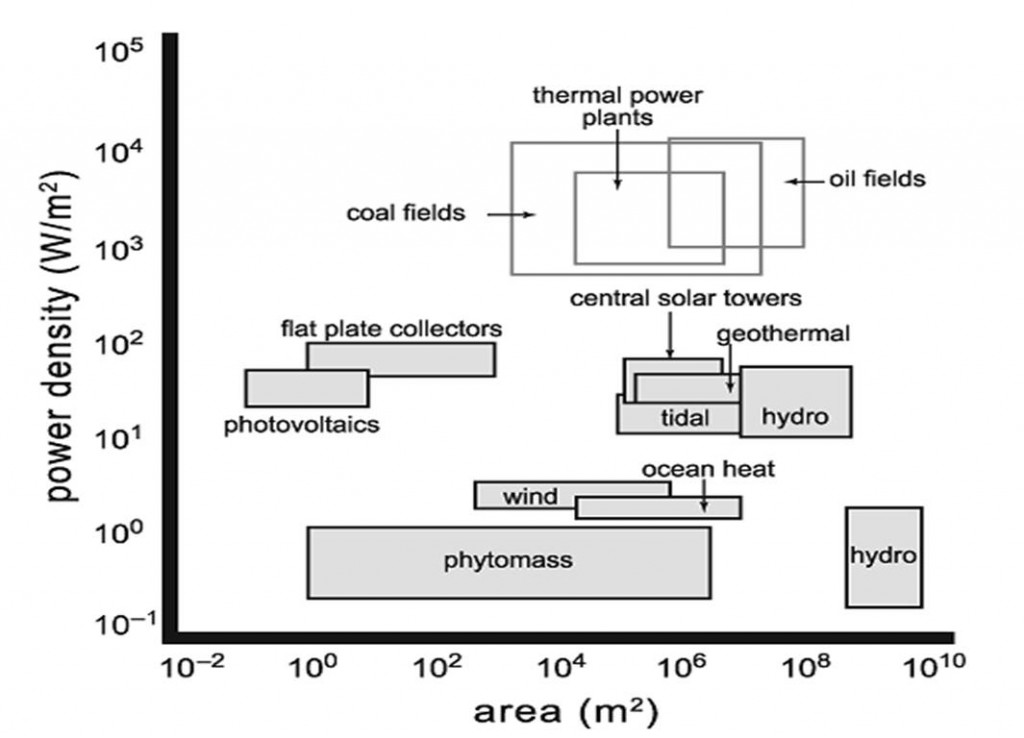
\includegraphics[width=1.00\textwidth]{graphics/Power-Densities.jpg}
	\caption{2222}
	\label{fig:Power-Densities}
\end{figure}




\section{Mining and Precious Metals}

\subsection{Gold in the Phillipines}

The Phillipines had the second largest gold reserve in world and employs approximately 200,000-300,000 people, most of who work in small scale mining operations, making approximately \$5/day (Pri)[??]

Many family miners, independent miners who make up the 70-80\% from small mining operations in the country. 


Large scale: \$70 billion 2014 (HWR)

90\% smuggled illegally

2015: Gov simplified process of gaining license 

But the Phillipines on just one region that has been subjected to the demand of gold and the re-occuring environmental and human tolls from the economic demand for gold. It drove some of the worst human behaviors from massacres, poisoning and destruction of whole groups of people via slavery and colonization. Although one could argue that the conditions today in the Phillipines is much better that the mines in the Andes or Brazil in the 1800s, but we would still be confronted with a terribly injustice system. To make a difference, we need to better appreciate why are these ores found unevenly and what are the processes to extract them and finally, how are the refined products used. 


\subsection{Geology and Gold}

\section{Mining and Proccesing Gold}

\subsection{Mining Methods and Ecological Impacts}

\subsection{Large Scale Processing}

\subsection{Smale Scale Operations}

\citet{drasch2001mt} \ldots

Working small scale in families... (Figure \ref{fig:famliymining}).

\begin{figure}[h]
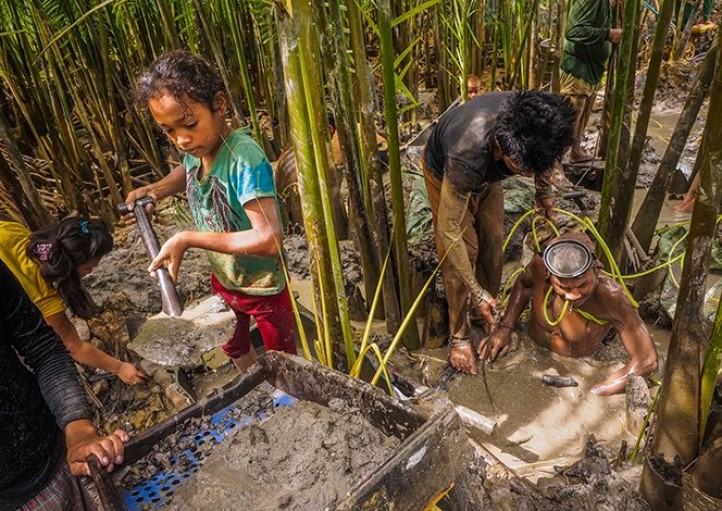
\includegraphics[width=\textwidth]{Family_Mining_Phillipines_SourceUnknwn}
\label{fig:famliymining}
\caption{Insert Caption Here: \ldots (With Permission ??).}
\end{figure}

\citep{de2016copper}

De la Torre, JB, Claveria RJ, Perez RE, Perez TR, Doronilla Al. 2016. Copper uptake by Pteris melanocaulon Fee from a Copper-Gold mine in Surigao del Norte Philippines. CRC Press LLC. 

Saludes, Mark. September 29, 2015. Hazardous Child Labor in Small-Scale Gold Mining in the Philippines. Human Rights Watch; [September 29, 2015; February 6, 2018].

\citet{santos1974mineral}

Santos G. 1974. Mineral Distribution and Geological Features of the Philippines. In: Petrascheck W.E. (eds) Metallogenetische und Geochemische Provinzen / Metallogenetic and Geochemical Provinces. �sterreichische Akademie der Wissenschaften Schriftenreihe der Erdwissenschaftlichen Kommission, vol 1. Springer, Vienna

Wernick, Adam. June 3, 2014. In the Philippines, underwater gold mining comes with small payoffs and big risk. PRI; [June 3, 2014; February 6, 2018]. 

\citet{drasch2001mt}

\section{Asia's Appetite for Sand}

Larson, Christina. "Asia's hunger for sand takes toll on ecology." (2018): 964-965.


%\bibliography{../references}



